\chapter{A Foray into Galactic Dynamics}
\newpage
%\section{Section}
%\subsection{SubSection}
%\subsubsection{SubSubSection}
%\paragraph{Paragraph}
%\subparagraph{SubParagraph}

\section{Perturbations to People}

Imagine you are standing on the corner of a busy Manhattan street. Every minute that passes shows the liveliness of a dynamic system, built up over many years. On an average block, there are approximately 28,154 people in the surrounding square kilometer, and a total of 1.7 million people on the island \citep{manhattan_population_density}. In contrast, a mere 300 years ago, the population was more disperse, and numbered in the thousands \citep{history_of_nyc}. From a collection of thousands of people in a relatively rarefied population formed a massive, dynamic ecosystem that represents an epicentre of modern human innovation and industry. Manhattan is not unique; cities across the world did not appear overnight, but were constructed hierarchically. It is in a similar fashion that modern astrophysics believes our Milky Way, and all massive galaxies formed with stars and gas as their building blocks.
\begin{figure}
	
\includegraphics[width=\textwidth]{../figures/2010_census}
	\caption{Population density information for the U.S. and Puerto Rico from the U.S. census bureau \citep{2010_us_census}}
\end{figure}

We believe that the Universe began with a period of rapid inflation, and that in the process of this inflation, pockets of the Universe emerged more dense than other regions. This is revealed to us through observations of the cosmic microwave background (CMB). The CMB is a portrait of the Universe when it was last opaque; before electrons, neutrons, and protons combined to form the first atoms. It shows temperature fluctations, like small population overdensities, that would eventually become cosmic cities.  While many physicists marvel at the physics that happens in these first moments of time, the story of how galaxies grow from cosmic villages contains many puzzles. This is the story of how tiny perturbations evolve to the structures astronomers see today, and it starts with the CMB.

When we look at the CMB, we are seeing the temperature distribution of matter through the radiation of baryonic matter, the matter that interacts with light. There is strong observational evidence to suggest that a large fraction of the matter present at this epoch is not interacting with light, including the power spectrum of the CMB itself \citep{transfer_fn}. The power spectrum describes the distribution of scales of the perturbations in the CMB, and presents some of the strongest evidence for the existence of dark matter, matter which does not interact with light.

Not only is there a measurable dark matter component in the Universe, it appears to be substantial. If the results from the Planck satellite are taken as truth, then dark matter comprises around 84\% of all matter in the Universe \citet{planck_2018}. Dark matter influences the evolution of galaxies not only because it is not subject to radiation-based interactions, but also because it is most of what there is. Dark matter is the glue that holds galaxies together.  

If dark matter is a glue, then dark energy is the opposite. Although dark matter makes up 84\% of the matter, matter only makes up 31.5\% of the present day Universe. The remainder is composed by a small contribution from radiation, but the bulk is comprised of this unaccounted for dark energy \citep{kolb_turner,dodelson}. Dark energy, whatever it is, is likely responsible for the observation of accelerating Universe expansion from Type 1a supernova measurements \citep{reiss_1998,perlmutter_1999}. Modern cosmology is a struggle between the competing forces of dark matter and dark energy, and both have implications for the local dynamics in the Universe.

A model of the Universe one might consider is one comprised of cold dark matter, that is dark matter which is massive and slow, and one which has dark energy, described on large scales by a single parameter, $\Lambda$. This paradigm is called $\Lambda$CDM and is the prevailing model in the astronomy community. The model has been enormously successful in explaining observations, including the CMB power spectrum. While there remain open problems with $\Lambda$CDM, it appears to predict many properties on Galactic and extragalactic scales correctly \citep{kolb_turner,dodelson}. Proposals to modify $\Lambda$CDM tend to present only slight variations on the model, such as allowing for self interacting dark matter (SIDM).
\begin{figure}
	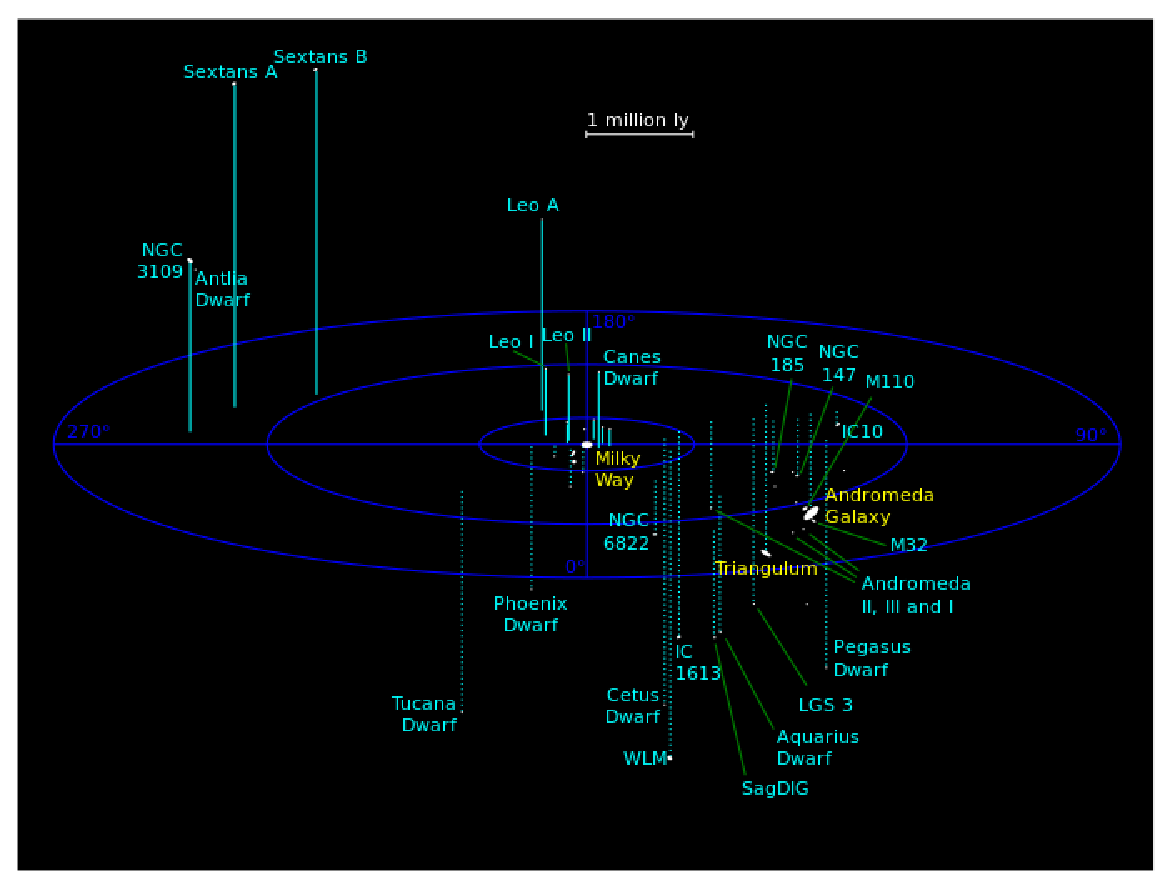
\includegraphics[width=\textwidth]{../figures/local_group}
	\caption{A map of the Local Group obtained per the license in \citet{local_group_map}.}\label{fig:local_group}
\end{figure}

Taking $\Lambda$CDM as the ground truth, the history of the Universe becomes understandable betweeen reionization and today. Dark matter, which does not interact through any force but gravity, retains a perturbed structure after inflation. The density perturbations collapse, forming potential wells of dark matter. The baryons, interacting through baryon acoustic oscillations (BOA), are delayed in falling into the potential wells made by the dark matter. As the baryons fall into the centers of the potential wells over time, the cores of the dark matter distributions, comprised of spheroidal units called halos, contract. After infall into a dark matter halo, the baryons cool to the point where stars are able to form. This is how the first galaxies formed.

Over time, galaxies begin to shift away from the linear mapping between perturbation and galaxy. Their forces on each other start to matter locally, and galaxies begin to merge hierarchically. Collections of galaxies form, sometimes massive clusters of $10^{15}$ solar masses. Other times, groups with a couple massive galaxies become host to many smaller galaxies called subhalos. Other galaxies belong to no group or cluster, and exist in the expansive void between clusters. Dark energy continues to pull the Universe apart, while locally galaxies are kept together by dark matter. Merging of galaxies continues on local scales as larger galaxies become larger, bringing us to today.

We live in a spiral galaxy of approximately $10^{12}$ solar masses (dark matter + baryons), in a group with another galaxy, M31 (Andromeda), which has a roughly similar mass. Our Local Group (Fig. \ref{fig:local_group}), as it is called, is comprised of many smaller galaxies. In our Milky Way's halo, for instance, a merger is beginning between the Milky Way and the Large and Small Magellanic Clouds (LMC/SMC), shown in the third quadrant of the inner circle around the Milky Way in Fig. \ref{fig:local_group}. The SMC/LMC systems total approximately 10-20\% of the Milky Way's mass in total \citep{erkal_lmc}. Most of our subhalos are not nearly this massive, although they number in the hundreds. The picture painted of the Local Group is that of M31 and the Milky Way devouring smaller galaxies. Of course, this will have a substantial impact on the evolution of the stars in the Milky Way, and is the crux of this thesis. By studying the Milky Way's local environment, we can hope to understand the interactions dark matter has on baryons, and perhaps infer something about how dark matter is distributed in our Galaxy.

%...the current de facto standard being the Unified Modeling Language
%(UML)~\cite{BRJ99}...

%\section{Problem}

%\section{Objective}

%\notesbox{Note:  These are the section headings that I decided to use.  Check out several
%recent theses to decide how you want to lay out your introduction (and conclusion) chapters.}


%\subsection{Hypothesis}

\section{Simulations as a Tool For Understanding Dark Matter Halos}

Many of the hardest questions in Galactic astrophysics stem from the fact that dark matter is not directly observable. As an example, what is the underlying smooth distribution of dark mass? How many dark matter subhalos should the Milky Way have? What is the effect on large scales if we choose something other than $\Lambda$CDM? While these questions are not easily answerable by direct observation, we can complement indirect observations with a solid theoretical understanding to reach some confident answers.

Simulations are the complementary theoretical understanding of galactic and extragalactic systems. When a simulation is performed, theoretical input is considered. This includes your model of cosmology, or your model of the galaxy, the nature of dark matter, etc. All of this knowledge is reduced to a fluid system which may be solved through numerical techniques on a computer.  When the results of a simulation are studied, we are studying the output of a given set of assumptions. In principle, this should allow us to evaluate whether or not cosmology is consistent with dynamics on a Galactic scale. $\Lambda$CDM has been tested in this way for decades, and we detail some global results in what follows.

We broadly commented on the hierarchical formation of galaxies. Over time, galaxies that merge with other galaxies should become well-mixed in the host halo. That is, there should be an underlying smooth distribution of mass in which all of the subhalos reside. A key prediction of $\Lambda$CDM is that this smooth distribution should have a universal density profile in the limit that dark matter dominates the Universe \citep{nfw}. Furthermore, the dark matter should have a density distribution somewhat resembling a squashed football, a spheroid flattened on two axes. Whether or not this picture holds observationally in real galaxies is an open problem. The density profile proposed by \citet{nfw} is cuspy at the center, whereas some observations are more consistent with a flatter central density \citep{de_block_core_cusp}. Astronomers have dubbed this the Core-Cusp Problem. From simply running a dark matter only simulation, we can infer the relative significance that baryonic physics plays in the central part of galaxies from these observational inconsistencies.

Despite the Core-Cusp Problem in the inner parts of dark matter haloes, one thing that is clear is that $\Lambda$CDM halos should have many subhalos.


\section{Response of Galactic Discs to the Environment}

Moving further down in scale from the Local Group we consider the state of a single galaxy, the Milky Way. While the Milky Way is by no means representative of every galaxy in the Universe, we have no reason to believe that it is particularly special. 


\section{Contributions}


\section{Organization of Thesis}

We proceed by introducing conformance checking and discussing related work in the next
chapter. We discuss the Alloy language and the Alloy Analyzer tool in
Chapter~\ref{ch:Alloy}.  Chapter~\ref{ch:Embee1} describes our Embee tool, from the
user's perspective, with several running examples.  Implementation details and the
analysis of the tool are presented in Chapter~\ref{ch:Embee2}.
Chapter~\ref{ch:Conclusion} concludes and outlines future work.

\bibliographystyle{apalike}
\bibliography{bibliography_introduction}